%%*************************************************************************
%% Legal Notice:
%% This code is offered as-is without any warranty either expressed or
%% implied; without even the implied warranty of MERCHANTABILITY or
%% FITNESS FOR A PARTICULAR PURPOSE! 
%% User assumes all risk.
%% In no event shall IEEE or any contributor to this code be liable for
%% any damages or losses, including, but not limited to, incidental,
%% consequential, or any other damages, resulting from the use or misuse
%% of any information contained here.
%%
%% All comments are the opinions of their respective authors and are not
%% necessarily endorsed by the IEEE.
%%
%% This work is distributed under the LaTeX Project Public License (LPPL)
%% ( http://www.latex-project.org/ ) version 1.3, and may be freely used,
%% distributed and modified. A copy of the LPPL, version 1.3, is included
%% in the base LaTeX documentation of all distributions of LaTeX released
%% 2003/12/01 or later.
%% Retain all contribution notices and credits.
%% ** Modified files should be clearly indicated as such, including  **
%% ** renaming them and changing author support contact information. **
%%
%% File list of work: IEEEtran.cls, IEEEtran_HOWTO.pdf, bare_adv.tex,
%%                    bare_conf.tex, bare_jrnl.tex, bare_jrnl_compsoc.tex
%%*************************************************************************

% *** Authors should verify (and, if needed, correct) their LaTeX system  ***
% *** with the testflow diagnostic prior to trusting their LaTeX platform ***
% *** with production work. IEEE's font choices can trigger bugs that do  ***
% *** not appear when using other class files.                            ***
% The testflow support page is at:
% http://www.michaelshell.org/tex/testflow/



% Note that the a4paper option is mainly intended so that authors in
% countries using A4 can easily print to A4 and see how their papers will
% look in print - the typesetting of the document will not typically be
% affected with changes in paper size (but the bottom and side margins will).
% Use the testflow package mentioned above to verify correct handling of
% both paper sizes by the user's LaTeX system.
%
% Also note that the "draftcls" or "draftclsnofoot", not "draft", option
% should be used if it is desired that the figures are to be displayed in
% draft mode.
%
\documentclass[conference]{IEEEtran}
% Add the compsoc option for Computer Society conferences.
%
% If IEEEtran.cls has not been installed into the LaTeX system files,
% manually specify the path to it like:
% \documentclass[conference]{../sty/IEEEtran}





% Some very useful LaTeX packages include:
% (uncomment the ones you want to load)


% *** MISC UTILITY PACKAGES ***
%
%\usepackage{ifpdf}
% Heiko Oberdiek's ifpdf.sty is very useful if you need conditional
% compilation based on whether the output is pdf or dvi.
% usage:
% \ifpdf
%   % pdf code
% \else
%   % dvi code
% \fi
% The latest version of ifpdf.sty can be obtained from:
% http://www.ctan.org/tex-archive/macros/latex/contrib/oberdiek/
% Also, note that IEEEtran.cls V1.7 and later provides a builtin
% \ifCLASSINFOpdf conditional that works the same way.
% When switching from latex to pdflatex and vice-versa, the compiler may
% have to be run twice to clear warning/error messages.






% *** CITATION PACKAGES ***
%
%\usepackage{cite}
% cite.sty was written by Donald Arseneau
% V1.6 and later of IEEEtran pre-defines the format of the cite.sty package
% \cite{} output to follow that of IEEE. Loading the cite package will
% result in citation numbers being automatically sorted and properly
% "compressed/ranged". e.g., [1], [9], [2], [7], [5], [6] without using
% cite.sty will become [1], [2], [5]--[7], [9] using cite.sty. cite.sty's
% \cite will automatically add leading space, if needed. Use cite.sty's
% noadjust option (cite.sty V3.8 and later) if you want to turn this off.
% cite.sty is already installed on most LaTeX systems. Be sure and use
% version 4.0 (2003-05-27) and later if using hyperref.sty. cite.sty does
% not currently provide for hyperlinked citations.
% The latest version can be obtained at:
% http://www.ctan.org/tex-archive/macros/latex/contrib/cite/
% The documentation is contained in the cite.sty file itself.






% *** GRAPHICS RELATED PACKAGES ***
%
\ifCLASSINFOpdf
\usepackage[pdftex]{graphicx}
  % declare the path(s) where your graphic files are
\graphicspath{{./images/}}
  % and their extensions so you won't have to specify these with
  % every instance of \includegraphics
\DeclareGraphicsExtensions{.jpg,.png}
\else
  % or other class option (dvipsone, dvipdf, if not using dvips). graphicx
  % will default to the driver specified in the system graphics.cfg if no
  % driver is specified.
  % \usepackage[dvips]{graphicx}
  % declare the path(s) where your graphic files are
  % \graphicspath{{../eps/}}
  % and their extensions so you won't have to specify these with
  % every instance of \includegraphics
  % \DeclareGraphicsExtensions{.eps}
\fi
% graphicx was written by David Carlisle and Sebastian Rahtz. It is
% required if you want graphics, photos, etc. graphicx.sty is already
% installed on most LaTeX systems. The latest version and documentation can
% be obtained at: 
% http://www.ctan.org/tex-archive/macros/latex/required/graphics/
% Another good source of documentation is "Using Imported Graphics in
% LaTeX2e" by Keith Reckdahl which can be found as epslatex.ps or
% epslatex.pdf at: http://www.ctan.org/tex-archive/info/
%
% latex, and pdflatex in dvi mode, support graphics in encapsulated
% postscript (.eps) format. pdflatex in pdf mode supports graphics
% in .pdf, .jpeg, .png and .mps (metapost) formats. Users should ensure
% that all non-photo figures use a vector format (.eps, .pdf, .mps) and
% not a bitmapped formats (.jpeg, .png). IEEE frowns on bitmapped formats
% which can result in "jaggedy"/blurry rendering of lines and letters as
% well as large increases in file sizes.
%
% You can find documentation about the pdfTeX application at:
% http://www.tug.org/applications/pdftex





% *** MATH PACKAGES ***
%
%\usepackage[cmex10]{amsmath}
% A popular package from the American Mathematical Society that provides
% many useful and powerful commands for dealing with mathematics. If using
% it, be sure to load this package with the cmex10 option to ensure that
% only type 1 fonts will utilized at all point sizes. Without this option,
% it is possible that some math symbols, particularly those within
% footnotes, will be rendered in bitmap form which will result in a
% document that can not be IEEE Xplore compliant!
%
% Also, note that the amsmath package sets \interdisplaylinepenalty to 10000
% thus preventing page breaks from occurring within multiline equations. Use:
%\interdisplaylinepenalty=2500
% after loading amsmath to restore such page breaks as IEEEtran.cls normally
% does. amsmath.sty is already installed on most LaTeX systems. The latest
% version and documentation can be obtained at:
% http://www.ctan.org/tex-archive/macros/latex/required/amslatex/math/





% *** SPECIALIZED LIST PACKAGES ***
%
%\usepackage{algorithmic}
% algorithmic.sty was written by Peter Williams and Rogerio Brito.
% This package provides an algorithmic environment fo describing algorithms.
% You can use the algorithmic environment in-text or within a figure
% environment to provide for a floating algorithm. Do NOT use the algorithm
% floating environment provided by algorithm.sty (by the same authors) or
% algorithm2e.sty (by Christophe Fiorio) as IEEE does not use dedicated
% algorithm float types and packages that provide these will not provide
% correct IEEE style captions. The latest version and documentation of
% algorithmic.sty can be obtained at:
% http://www.ctan.org/tex-archive/macros/latex/contrib/algorithms/
% There is also a support site at:
% http://algorithms.berlios.de/index.html
% Also of interest may be the (relatively newer and more customizable)
% algorithmicx.sty package by Szasz Janos:
% http://www.ctan.org/tex-archive/macros/latex/contrib/algorithmicx/




% *** ALIGNMENT PACKAGES ***
%
%\usepackage{array}
% Frank Mittelbach's and David Carlisle's array.sty patches and improves
% the standard LaTeX2e array and tabular environments to provide better
% appearance and additional user controls. As the default LaTeX2e table
% generation code is lacking to the point of almost being broken with
% respect to the quality of the end results, all users are strongly
% advised to use an enhanced (at the very least that provided by array.sty)
% set of table tools. array.sty is already installed on most systems. The
% latest version and documentation can be obtained at:
% http://www.ctan.org/tex-archive/macros/latex/required/tools/


%\usepackage{mdwmath}
%\usepackage{mdwtab}
% Also highly recommended is Mark Wooding's extremely powerful MDW tools,
% especially mdwmath.sty and mdwtab.sty which are used to format equations
% and tables, respectively. The MDWtools set is already installed on most
% LaTeX systems. The lastest version and documentation is available at:
% http://www.ctan.org/tex-archive/macros/latex/contrib/mdwtools/


% IEEEtran contains the IEEEeqnarray family of commands that can be used to
% generate multiline equations as well as matrices, tables, etc., of high
% quality.


%\usepackage{eqparbox}
% Also of notable interest is Scott Pakin's eqparbox package for creating
% (automatically sized) equal width boxes - aka "natural width parboxes".
% Available at:
% http://www.ctan.org/tex-archive/macros/latex/contrib/eqparbox/





% *** SUBFIGURE PACKAGES ***
%\usepackage[tight,footnotesize]{subfigure}
% subfigure.sty was written by Steven Douglas Cochran. This package makes it
% easy to put subfigures in your figures. e.g., "Figure 1a and 1b". For IEEE
% work, it is a good idea to load it with the tight package option to reduce
% the amount of white space around the subfigures. subfigure.sty is already
% installed on most LaTeX systems. The latest version and documentation can
% be obtained at:
% http://www.ctan.org/tex-archive/obsolete/macros/latex/contrib/subfigure/
% subfigure.sty has been superceeded by subfig.sty.



%\usepackage[caption=false]{caption}
%\usepackage[font=footnotesize]{subfig}
% subfig.sty, also written by Steven Douglas Cochran, is the modern
% replacement for subfigure.sty. However, subfig.sty requires and
% automatically loads Axel Sommerfeldt's caption.sty which will override
% IEEEtran.cls handling of captions and this will result in nonIEEE style
% figure/table captions. To prevent this problem, be sure and preload
% caption.sty with its "caption=false" package option. This is will preserve
% IEEEtran.cls handing of captions. Version 1.3 (2005/06/28) and later 
% (recommended due to many improvements over 1.2) of subfig.sty supports
% the caption=false option directly:
%\usepackage[caption=false,font=footnotesize]{subfig}
%
% The latest version and documentation can be obtained at:
% http://www.ctan.org/tex-archive/macros/latex/contrib/subfig/
% The latest version and documentation of caption.sty can be obtained at:
% http://www.ctan.org/tex-archive/macros/latex/contrib/caption/




% *** FLOAT PACKAGES ***
%
%\usepackage{fixltx2e}
% fixltx2e, the successor to the earlier fix2col.sty, was written by
% Frank Mittelbach and David Carlisle. This package corrects a few problems
% in the LaTeX2e kernel, the most notable of which is that in current
% LaTeX2e releases, the ordering of single and double column floats is not
% guaranteed to be preserved. Thus, an unpatched LaTeX2e can allow a
% single column figure to be placed prior to an earlier double column
% figure. The latest version and documentation can be found at:
% http://www.ctan.org/tex-archive/macros/latex/base/



\usepackage{stfloats}
% stfloats.sty was written by Sigitas Tolusis. This package gives LaTeX2e
% the ability to do double column floats at the bottom of the page as well
% as the top. (e.g., "\begin{figure*}[!b]" is not normally possible in
% LaTeX2e). It also provides a command:
%\fnbelowfloat
% to enable the placement of footnotes below bottom floats (the standard
% LaTeX2e kernel puts them above bottom floats). This is an invasive package
% which rewrites many portions of the LaTeX2e float routines. It may not work
% with other packages that modify the LaTeX2e float routines. The latest
% version and documentation can be obtained at:
% http://www.ctan.org/tex-archive/macros/latex/contrib/sttools/
% Documentation is contained in the stfloats.sty comments as well as in the
% presfull.pdf file. Do not use the stfloats baselinefloat ability as IEEE
% does not allow \baselineskip to stretch. Authors submitting work to the
% IEEE should note that IEEE rarely uses double column equations and
% that authors should try to avoid such use. Do not be tempted to use the
% cuted.sty or midfloat.sty packages (also by Sigitas Tolusis) as IEEE does
% not format its papers in such ways.





% *** PDF, URL AND HYPERLINK PACKAGES ***
%
%\usepackage{url}
% url.sty was written by Donald Arseneau. It provides better support for
% handling and breaking URLs. url.sty is already installed on most LaTeX
% systems. The latest version can be obtained at:
% http://www.ctan.org/tex-archive/macros/latex/contrib/misc/
% Read the url.sty source comments for usage information. Basically,
% \url{my_url_here}.





% *** Do not adjust lengths that control margins, column widths, etc. ***
% *** Do not use packages that alter fonts (such as pslatex).         ***
% There should be no need to do such things with IEEEtran.cls V1.6 and later.
% (Unless specifically asked to do so by the journal or conference you plan
% to submit to, of course. )


% correct bad hyphenation here
\hyphenation{op-tical net-works semi-conduc-tor}

\begin{document}
%
% paper title
% can use linebreaks \\ within to get better formatting as desired
\title{A Blocks-Based Editor for HTML Code}

% author names and affiliations
% use a multiple column layout for up to three different
% affiliations
\author{
\IEEEauthorblockN{Saksham Aggarwal}
\IEEEauthorblockA{International Institute of Information Technology\\
Hyderabad, India\\
saksham.aggarwal@students.iiit.ac.in}
\and
\IEEEauthorblockN{David Anthony Bau}
\IEEEauthorblockA{Phillips Exeter Academy\\
Exeter, NH, USA\\
dbau@exeter.edu}
\and
\IEEEauthorblockN{David Bau}
\IEEEauthorblockA{Google\\
Cambridge, MA, USA\\
davidbau@google.com}
}

% conference papers do not typically use \thanks and this command
% is locked out in conference mode. If really needed, such as for
% the acknowledgment of grants, issue a \IEEEoverridecommandlockouts
% after \documentclass

% for over three affiliations, or if they all won't fit within the width
% of the page, use this alternative format:
% 
%\author{\IEEEauthorblockN{Michael Shell\IEEEauthorrefmark{1},
%Homer Simpson\IEEEauthorrefmark{2},
%James Kirk\IEEEauthorrefmark{3}, 
%Montgomery Scott\IEEEauthorrefmark{3} and
%Eldon Tyrell\IEEEauthorrefmark{4}}
%\IEEEauthorblockA{\IEEEauthorrefmark{1}School of Electrical and Computer Engineering\\
%Georgia Institute of Technology,
%Atlanta, Georgia 30332--0250\\ Email: see http://www.michaelshell.org/contact.html}
%\IEEEauthorblockA{\IEEEauthorrefmark{2}Twentieth Century Fox, Springfield, USA\\
%Email: homer@thesimpsons.com}
%\IEEEauthorblockA{\IEEEauthorrefmark{3}Starfleet Academy, San Francisco, California 96678-2391\\
%Telephone: (800) 555--1212, Fax: (888) 555--1212}
%\IEEEauthorblockA{\IEEEauthorrefmark{4}Tyrell Inc., 123 Replicant Street, Los Angeles, California 90210--4321}}




% use for special paper notices
%\IEEEspecialpapernotice{(Invited Paper)}




% make the title area
\maketitle


\begin{abstract}
%\boldmath
This paper presents a block-programming editor for HTML code.  The editor provides a block visualization of HTML syntax, allowing students to work in either blocks or text and switch freely.  Our editor was created as an extension of Droplet, a dual-mode programming block editing framework that was previously used for JavaScript and CoffeeScript. We describe the process of extending Droplet to apply to HTML. We also discuss an analysis of real-world HTML tags and attributes and propose a palette based on this analysis.

\end{abstract}
% IEEEtran.cls defaults to using nonbold math in the Abstract.
% This preserves the distinction between vectors and scalars. However,
% if the conference you are submitting to favors bold math in the abstract,
% then you can use LaTeX's standard command \boldmath at the very start
% of the abstract to achieve this. Many IEEE journals/conferences frown on
% math in the abstract anyway.

% no keywords




% For peer review papers, you can put extra information on the cover
% page as needed:
% \ifCLASSOPTIONpeerreview
% \begin{center} \bfseries EDICS Category: 3-BBND \end{center}
% \fi
%
% For peerreview papers, this IEEEtran command inserts a page break and
% creates the second title. It will be ignored for other modes.
\IEEEpeerreviewmaketitle

\section{Introduction}
Teaching HTML has long been an early step in a programming curriculum.  For example Budny, et al \cite{Budny} in Four Steps to Teaching C Programming, suggest ``The layout of a web page allowed us to begin to teach the basic concepts of program layout... We are teaching web page design ... not for the purpose of teaching HTML, but to teach students the concept of writing code.'' Mahmoud, et al \cite{Mahmoud} suggest that starting with HTML is a way of teaching ``programming for fun'' and is a strategy for motivating students.

Nonetheless, for first-time-coder, HTML can be difficult to learn.  In a workshop with English students, Mauriello, Pagnucci, and Winner \cite{Mauriello} observed ``Students are generally not careful and experienced enough in their reading of the codes to find mistakes.''  HTML guides for non-coding students such as Taylor and Gitsaki \cite{Taylor} suggest simplifying the problem by starting with a small set of about 30 HTML tags to create a basic web page.

Therefore we are interested in finding an alternative to WYSIWYG HTML tools that expose the code, while still simplifying the process of learning to use HTML tags for the first time.  In recent years, block programming languages such as Scratch \cite{Scratch} have introduced many students to coding through a visual representation of commands and control flow.  Here we investigate whether a similar approach can be used with HTML code.

We aim to meet three goals simultaneously (borrowing terminology from Nielsen's usability heuristics\cite{Nielsen}):

\begin{itemize}
\item Allow students to create HTML using \emph{recognition rather than recall}, assembling blocks to make pages.
\item Permit editing of real-world wepages with blocks or text: \emph{the system must match the real world}.
\item Provide students with a \emph{minimalist design} with a clear, useful, realistic, yet minimal set of choices.
\end{itemize}


\section{Background}

\subsection{Droplet's Text-First Approach to Blocks}

\begin{figure}
\centering
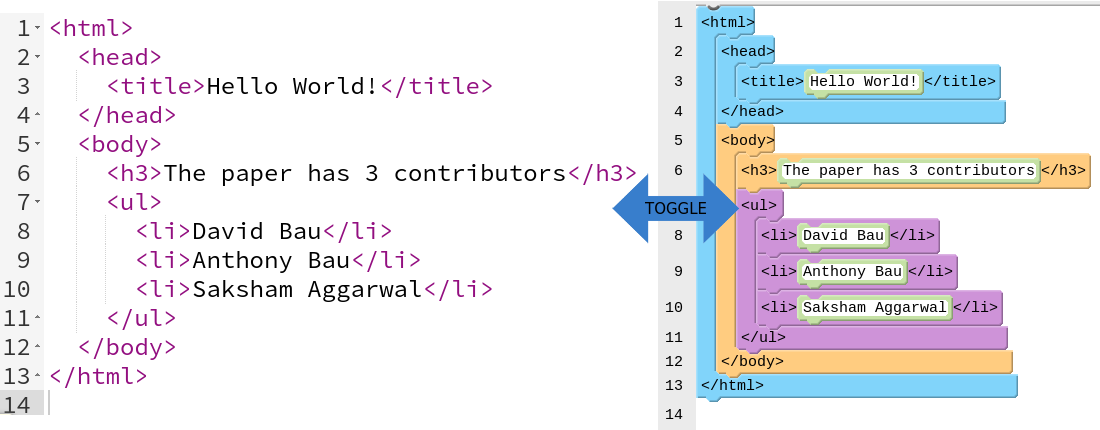
\includegraphics[width=\columnwidth]{dualmode.png}
\caption{Our HTML Block editor user experience}
\small
\begin{flushleft}
Users can switch between blocks and text freely.
\end{flushleft}
\label{dropletimage}
\end{figure}

We built our HTML editor as an extension of Droplet.  Droplet \cite{Droplet} is a dual-mode blocks and text editor framework that allows students to work with traditional text code syntax using either drag-and-drop blocks or by typing the text.  Students can switch modes at any time.

Droplet's guiding philosophy is that the text, not the blocks, are the primary data. Thus, Droplet programs begin and end their life as text. When Droplet opens a file, the text is parsed into blocks, preserving the original text within block markup. Block editing operations perform splice operations on the text markup stream. At the end of the editing session, the markup is simply discarded and a raw text program is generated again. Figure \ref{dropletimage} shows a typical droplet user experience for our HTML editor, and Figure \ref{lifecycle} shows the lifecycle of a Droplet program.

\begin{figure}
\centering
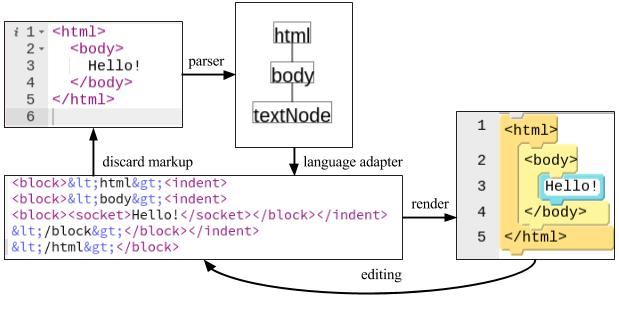
\includegraphics[width=0.5\columnwidth]{lifecycle.jpg}
\caption{Lifecycle of a Droplet Editing Session}
\label{lifecycle}
\end{figure}

\subsection{Adding A New Language to Droplet}

Droplet is designed to be extended to any text language by creating a language adapter.

A Droplet language adapter must parse text to delinate blocks, and it can also provide rules that determine whether blocks are allowed to be dropped into specific locations.  Typically the language parser relies on a standard language parser, inserting blocks based on positions of specific types of nodes in an AST.  Callback functions are used to determine drag-and-drop permissibility.

New languages in Droplet also need a block palette.  The Droplet palette is a reflection of useful choices, not a complete catalog of all possible blocks for a language.  Similarly, dropdown choices for for sockets within blocks are curated suggestions.  Users are always free to enter tags and attributes as free-form text, but a good palette design will allow all he common cases to be handled with drag-and-drop.

\section{Process}

\subsection{Adapting A Parser}

One of the goals of our HTML editor is to be able to visualize real-world webpages as blocks. This poses a difficulty because browsers are tolerant and many existing webpages are not strictly standards-compliant, with mismatched tags, and missing, implicit, or redundant elements.

Droplet's HTML mode adapts the parse5 HTML parser \cite{parse5}, which tolerates syntactically ``incorrect'' HTML code in the same way browsers do. We modified the parse5 parser for Droplet's purposes to add more detailed location data, so that precise source code locations for tags can be extracted.

The block parsing process for HTML proceeds as the following psuedocode:
\begin{enumerate}
  \item Parse the text into an DOM tree using parse5.
  \item Process the root of the DOM.
  \item For each node, check if it is a text node, comment, empty element or an element with content.
  \item Mark the range of a node based on its type
  \begin{itemize}
    \item If a text node, make it editable.
    \item If a comment, make the comment editable.
    \item If an empty element, mark it as a block and make its attributes editable.
    \item If an element with content, mark it as a block, make its attributes editable and add an indent to make space for its children.
    \item If an implicit or error tag, do not mark it.
  \end{itemize}
  \item Recurse from step (3) for every child.
\end{enumerate}

\subsection{Enforcing Droppability Rules}

One major advantage of a block language is that it can guide authoring so that students create standards-compliant code. Droplet's HTML mode therefore enforces droppability rules adapted from the WHATWG HTML specifications \cite{WHATWG}.  For example, a \texttt{<head>} element may only contain metadata elements such as \texttt{<title>} and \texttt{<meta>}, and a \texttt{<table>} element may only contain appropriate table elements such as \texttt{<tr>} and \texttt{<colgroup>} and \texttt{<caption>}.

We have implemented standard the containment rules for 92 tags.  When a block is dragged into the document, only legal locations according to these rules are highlighted, and when a drop occurs, only those locations will receive a block.

\subsection{Choosing A Palette}

The palette in a block language is important to discovery and self-directed learning, because students can try new commands without having to read documentation. Having a palette that contains useful and rewarding tags in an HTML mode is therefore important.

The WHATWG HTML specifications define over 100 tags. However, most them are not used on a typical webpage. A number of developers online have informally posted HTML cheat sheets with the ``most important tags,'' \cite{Webmonkey} \cite{SimpleGuide} \cite{Usabilla} but these are subjective and often conflict with each other. Because Droplet's philosophy is to be able to interact with real-world code on the Internet, we here determine and recommend a palette based on real-world tag frequencies.

We are not aware of any published statistics on the real-world frequency of HTML tag usage on the web, so we crawled a selection of 52460 webpages using Common Crawl \cite{commoncrawl} to create real-world frequency data. Our analysis of the top 108 tags is summarized in Figure \ref{Tagsgraph}.  (Full data from our crawl is available on github \cite{FullResults}.)  Red bars in that graph represent a count of the number of times each tag was used per page on average in the crawled data set.  The blue line, on a logarithmic scale, represents the percentage of documents in the data set that used the tag.  In addition, we analyzed the most common tag-attribute pairs.  These statistics are summarized in Figure \ref{attrgraph}.  Red bars on that graph represent the percentage of webpages that include a given attribute on a specific tag.

\begin{figure}
\centering
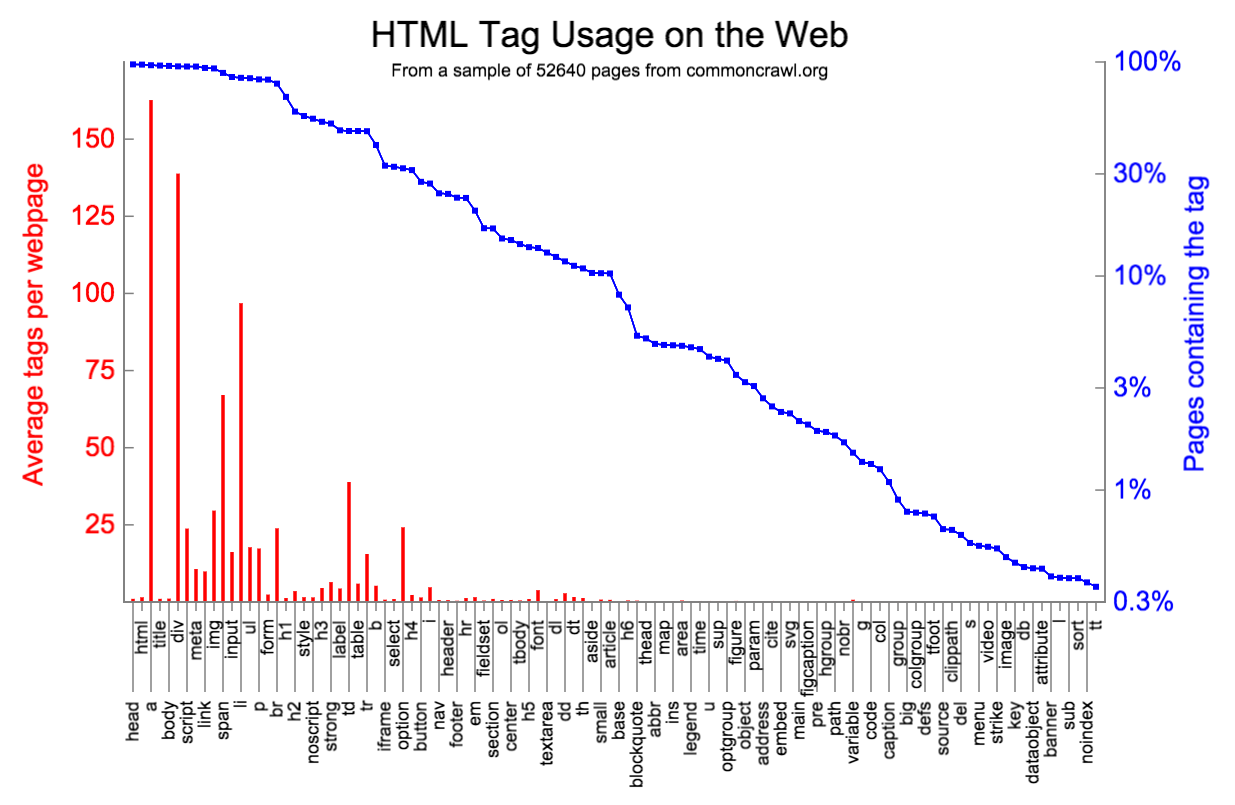
\includegraphics[width=\columnwidth]{taggraph3.png}
\caption{HTML Tag Usage on the Web}
\label{Tagsgraph}
\end{figure}

\begin{figure}
\centering
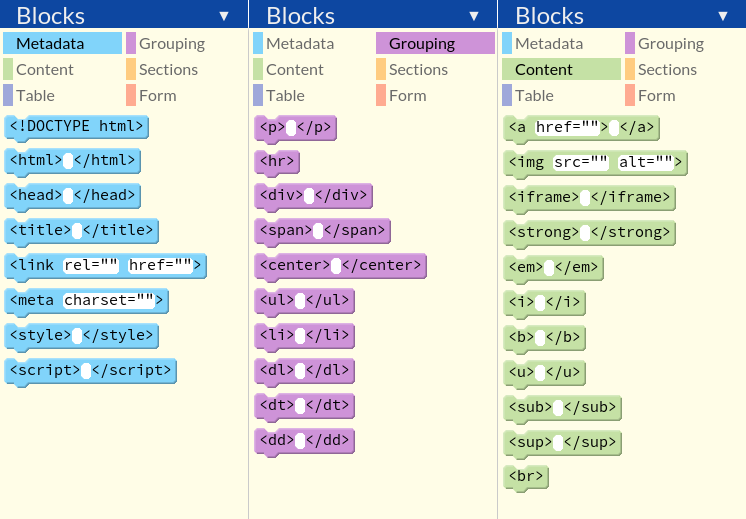
\includegraphics[width=0.7\columnwidth]{Palette.png}
\caption{Three panels from the palette}
\label{paletteimage}
\end{figure}

\begin{figure}
\centering
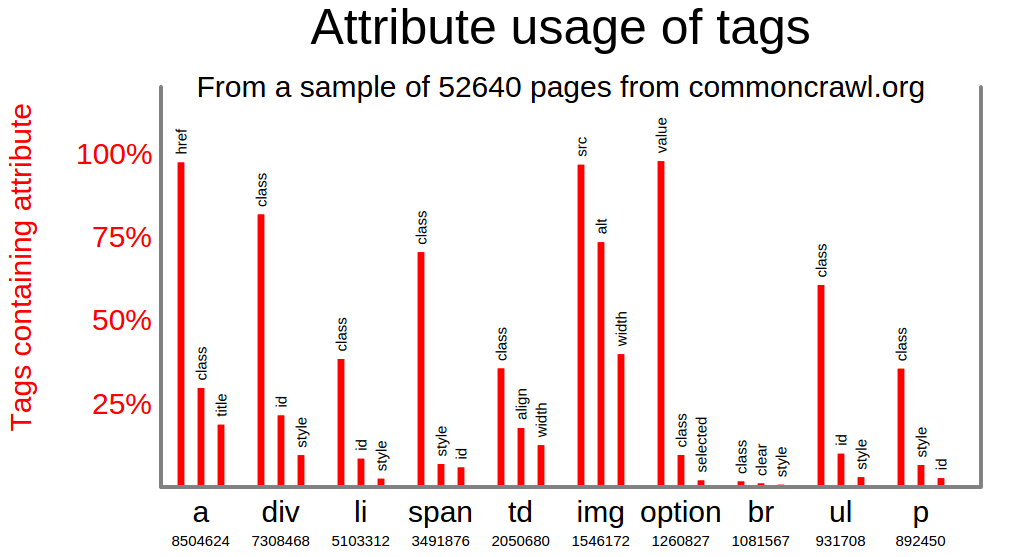
\includegraphics[width=\columnwidth]{attrgraph.png}
\caption{Top attributes used with tags}
\label{attrgraph}
\end{figure}

\begin{figure}
\centering
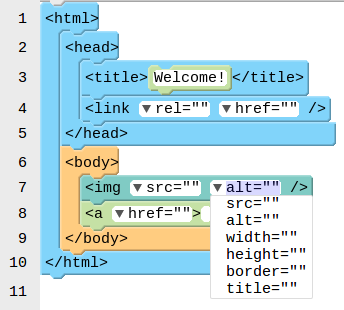
\includegraphics[width=0.5\columnwidth]{dropdown.png}
\caption{Using commonly used attributes in a dropdown}
\label{dropdownimage}
\end{figure}

We created the final palette (Figure \ref{paletteimage}) by choosing the top 40 tags from the above 2 analysis results, adding a few elements to align with courses such as \cite{htmltutor1} \cite{htmltutor2} \cite{htmltutor3}, and removing some elements which have a similar behavior as another commonly-used alternative such as \texttt{<i>} versus \texttt{<em>}.

We also created dropdown lists for each element (Figure \ref{dropdownimage}) to allow stduents to choose between the most common attributes.  The student can choose an attribute and enter the attribute value as text, or just enter the entire attribute/value pair as text.

\section{Future Work}

\subsection{Buttons for adding and removing attributes}
In HTML, every tag can accept a variable number of attributes, and the HTML mode would benefit from improved block editor support for variable argument lists.  We are building improvements to make it easy to use ``add/remove'' buttons on a block for adding new attributes.

\subsection{Polymorphic elements}
Some elements are used in several distinct ways, and we plan to do further analysis on common tag usage to decide on a few tags to represent in multiple ways on the palette.  For example, two ways of using \texttt{<a>} are with \texttt{href} or with \texttt{name}; two ways of using \texttt{<script>} are with \texttt{src} or with inline script.

\subsection{Transparent content model}
Some tags such as `a', `ins', `del', `map' are ``transparent'' elements, which means, according to the standard \cite{whatwgtransparent}, their content model is derived from the content model of its parent element. This type of contextual content model is not currently implemented but provided as ``flow content'' \cite{flowcontent}.  We plan to add support for a transparent content model.

\section*{Acknowledgement}

We are grateful to Google Summer of Code, which supported Saksham Aggarwal's open-source work on this project.

\begin{thebibliography}{1}

\bibitem{Budny}
  Budny, D.; Lund, L.; Vipperman, J.; Patzer, J.L.I.I.I., ``Four steps to teaching C programming,'' Frontiers in Education, 2002. FIE 2002. 32nd Annual , vol.2, no., pp.F1G-18,F1G-22 vol.2, 2002
\bibitem{Mahmoud}
  Qusay H. Mahmoud, Wlodek Dobosiewicz, and David Swayne. 2004. Redesigning introductory computer programming with HTML, JavaScript, and Java. SIGCSE Bull. 36, 1 (March 2004), 120-124. DOI=10.1145/1028174.971344 http://doi.acm.org/10.1145/1028174.971344
\bibitem{Mauriello}
  Mauriello, N. Pagnucci, G. and Winner, T. Reading between the Code: The Teaching of HTML and the Displacement of Writing Instruction. Computers and Composition 16, 409-19 (1999)
\bibitem{Taylor}
  Taylor, R. and Gitaski, C. Teaching WELL and loving IT. New Perspectives on CALL for Second Language Classrooms, 131-147.
\bibitem{Scratch}
  Scratch. https://scratch.mit.edu/
\bibitem{Nielsen}
  Nielsen, Jakob. Usability engineering. Elsevier, 1994.
\bibitem{Droplet}
  Bau, D. A. Droplet, A Blocks-Based Editor for Text Code. Journal of Computer Science in Colleges. 30, 6 (June 2015).
\bibitem{parse5}
  Parse5. https://github.com/inikulin/parse5
\bibitem{WHATWG}
  HTML living standard. https://html.spec.whatwg.org/
\bibitem{FullResults}
  https://github.com/sakagg/HTMLtagsFrequencyAnalysis
\bibitem{commoncrawl}
  Common Crawl. https://commoncrawl.org/
\bibitem{pencilcodehtml}
  HTML Palette in use on Pencil Code. pencilcode.net/edit/example.html
\bibitem{Webmonkey}
  Webmonkey. HTML Cheat Sheet.\\ http://www.webmonkey.com/2010/02/html\_cheatsheet/
\bibitem{SimpleGuide}
  A Simple Guide to HTML. HTML Cheat Sheet.\\ http://www.simplehtmlguide.com/cheatsheet.php
\bibitem{Usabilla}
  Usabilla. An HTML Cheat Sheet That Never Fails. http://blog.usabilla.com/an-html-cheat-sheet-that-never-fails/
\bibitem{htmltutor1}
  Exploring computer Science - pages 105-110\\
  http://www.exploringcs.org/wp-content/uploads/2014/02/ExploringComputerScience-v5.0.pdf
\bibitem{htmltutor2}
  W3Schools HTML starters guide\\
  http://www.w3schools.com/html/default.asp
\bibitem{htmltutor3}
  Htmldog beginner tutorial http://htmldog.com/guides/html/beginner/conclusion/
\bibitem{flowcontent}
  WHATWG flow content list\\
  https://developers.whatwg.org/content-models.html\#flow-content
\bibitem{metadata}
  WHATWG metadata content list\\
  https://developers.whatwg.org/content-models.html\#metadata-content
\bibitem{phrasing}
  WHATWG phrasing content list\\
  https://developers.whatwg.org/content-models.html\#phrasing-content
\bibitem{interactive}
  WHATWG interactive content list\\
  https://developers.whatwg.org/content-models.html\#interactive-content
\bibitem{script}
  WHATWG script supporting elements\\
  https://developers.whatwg.org/content-models.html\#script-supporting-elements
\bibitem{whatwgtransparent}
  https://html.spec.whatwg.org/multipage/dom.html\#transparent-content-models

\end{thebibliography}

% that's all folks
\end{document}
